% ============================================================================
% SCAI 2026 Poster - A0 Portrait
% OCR and Machine Translation Pipeline for Low-Resource Sami Languages
% Based on tikzposter, follows SCAI 2026 PosterGuidelines:
%   - A0 portrait (84.1 x 118.9 cm)
%   - Title 72-100pt, headings 36-48pt, body 24-32pt, captions 18-24pt
%   - 3-4 column layout, prefer visuals, high contrast, readable from 1-2 m
% ============================================================================
\documentclass[30pt, a0paper, portrait,
               margin=0mm, innermargin=15mm,
               blockverticalspace=12mm, colspace=15mm, subcolspace=8mm]{tikzposter}

\usepackage[T1]{fontenc}
\usepackage[utf8]{inputenc}
\usepackage{lmodern}
\usepackage{graphicx}
\usepackage{array}
\usepackage{booktabs}
\usepackage{multirow}
\usepackage{amsmath}
\usepackage{xcolor}
\usepackage{hyperref}
\usepackage{enumitem}
\setlist{nosep,leftmargin=*}

\usepackage{caption}
\captionsetup{font=footnotesize}

% ============================================================================
% BENCHMARK MACROS - synced with scai_paper/main.tex
% ============================================================================
\newcommand{\ctcCER}{12.24}
\newcommand{\ctcWER}{37.35}
\newcommand{\ctcCacc}{87.72}
\newcommand{\ctcWordAcc}{62.65}
\newcommand{\ctcTime}{0.033}
\newcommand{\modelSize}{23MB}

\newcommand{\trocrBestCER}{8.55}
\newcommand{\trocrBestWER}{28.16}
\newcommand{\trocrBestCacc}{91.56}
\newcommand{\trocrBestWordAcc}{71.84}
\newcommand{\trocrBestTime}{12.41}
\newcommand{\trocrSize}{350MB}

\newcommand{\trocrPredSynthCharAcc}{84.15}
\newcommand{\trocrPredSynthWordAcc}{54.24}
\newcommand{\trocrPredSynthTime}{12.08}
\newcommand{\trocrSmiCharAcc}{75.88}
\newcommand{\trocrSmiWordAcc}{36.50}
\newcommand{\trocrSmiTime}{16.23}

\newcommand{\bleuScore}{10.40}
\newcommand{\chrfScore}{33.85}
\newcommand{\terScore}{76.30}

\newcommand{\speedupFactor}{380}
\newcommand{\sizeRatio}{15}
\newcommand{\cerAccGap}{3.84}
\newcommand{\throughputCtc}{109{,}000}
\newcommand{\throughputTrocr}{290}

\newcommand{\benchmarkSamples}{1048}
\newcommand{\hfTestSamples}{1000}
\newcommand{\bookTestSamples}{48}

% Conjunction-based splitting (long sentences > sentenceLengthThreshold)
\newcommand{\splitLongOriginalCER}{15.17}
\newcommand{\splitLongSplitCER}{8.12}
\newcommand{\splitShortCER}{12.04}

% Domain-specific CER (in-domain HuggingFace vs. out-of-domain book text)
\newcommand{\trocrSynthHFCER}{8.33}
\newcommand{\trocrSynthBookCER}{13.17}
\newcommand{\trocrSynthDeltaCER}{4.84}
\newcommand{\ctcBookCER}{12.21}
\newcommand{\trocrPredSynthHFCER}{16.09}
\newcommand{\trocrPredSynthBookCER}{11.00}
\newcommand{\trocrPredSynthDeltaCER}{5.09}

% ============================================================================
% THEME / COLORS -- pure SDU black-and-white
% Every tikzposter colour is explicitly overridden, so the underlying
% colorstyle ("Default") only acts as a neutral base.
% ============================================================================
\usetheme{Simple}
\usecolorstyle{Default}
% Custom blockstyle: same as Default, but with a noticeable corner radius
% so the rounded shape reads at A0 distance.
\defineblockstyle{SduRounded}{%
    titlewidthscale=1, bodywidthscale=1, titleleft,
    titleoffsetx=0pt, titleoffsety=0pt,
    bodyoffsetx=0pt,  bodyoffsety=15pt,
    bodyverticalshift=10pt, roundedcorners=30, linewidth=2pt,
    titleinnersep=8mm, bodyinnersep=1cm
}{%
    \draw[color=framecolor, fill=blockbodybgcolor,
          rounded corners=\blockroundedcorners]
          (blockbody.south west) rectangle (blockbody.north east);
    \ifBlockHasTitle
        \draw[color=framecolor, fill=blocktitlebgcolor,
              rounded corners=\blockroundedcorners]
              (blocktitle.south west) rectangle (blocktitle.north east);
    \fi
}
\useblockstyle{SduRounded}
\colorlet{backgroundcolor}{white}
\colorlet{framecolor}{black}
\colorlet{titlebgcolor}{white}
\colorlet{titlefgcolor}{black}
\colorlet{blocktitlebgcolor}{black}
\colorlet{blocktitlefgcolor}{white}
\colorlet{blockbodybgcolor}{white}
\colorlet{blockbodyfgcolor}{black}
\colorlet{innerblocktitlebgcolor}{black!10}
\colorlet{innerblocktitlefgcolor}{black}
\colorlet{notebgcolor}{black!5}
\colorlet{notefrcolor}{black}
% Remove the tikzposter watermark / background gradient
\tikzposterlatexaffectionproofoff

% ============================================================================
% TITLE BLOCK
% ============================================================================
\title{\parbox{\linewidth}{\centering OCR and Machine Translation Pipeline\\
       for Low-Resource S\'{a}mi Languages}}
\author{Jan Paweł Musioł\textsuperscript{1} \quad Aparna S. Varde\textsuperscript{2} \quad Juan Heredia\textsuperscript{3}}
\institute{University of Southern Denmark --- \textsuperscript{1}S\o nderborg \quad \textsuperscript{2}Vejle \quad \textsuperscript{3}Odense, Denmark\\
\texttt{jamus23@student.sdu.dk} \quad \texttt{\{apva,jehm\}@mmmi.sdu.dk}}

% Custom title layout: SCAI logo (left) | title block (centre) | SDU logo (right)
\settitle{%
  \centering
  \begin{minipage}[c]{0.10\linewidth}\centering
    
\includegraphics[width=\linewidth]{figures/logo-scai-2-400x400px.jpg}%
  \end{minipage}\hfill
  \begin{minipage}[c]{0.70\linewidth}\centering
    {\color{titlefgcolor}\bfseries\Huge \@title \par}
    \vspace*{0.8em}
    {\Large \@author \par}
    \vspace*{0.4em}
    {\large \@institute \par}
  \end{minipage}\hfill
  \begin{minipage}[c]{0.10\linewidth}\centering
    
\includegraphics[width=\linewidth]{figures/sdu_logo.pdf}%
  \end{minipage}%
}

\begin{document}

\maketitle[width=\textwidth, titletotopverticalspace=10mm,
           titletoblockverticalspace=15mm]

% ============================================================================
% ROW 1 -- 3 COLUMNS
% ============================================================================
\begin{columns}

% ------------------------------ COLUMN 1 ------------------------------
\column{0.33}

% Introduction / Background
% o Research context
% o Motivation
% o Objectives
\block{1.\ Background \& Motivation}{
\textbf{S\'{a}mi languages} are a group of nine low-resource Uralic languages spoken across Northern Europe. Northern S\'{a}mi, the most widely spoken, has approximately $25{,}000$ speakers and is classified as endangered by UNESCO.

\textbf{Challenges} in Optical Character Recognition (OCR) for North S\'{a}mi range from scarce training data to complex orthographic features, making it a difficult task to streamline the digitalization efforts. Additionally, the language characteristics of S\'{a}mi lead to a large number of inflected word forms, further complicating accurate recognition. While state-of-the-art models like TrOCR achieve high accuracy (\trocrBestCacc\%), their computational demands ($\sim$\trocrSize, $\sim$\trocrBestTime\,s/img inference on CPU) make them ill-fitted for deployment in resource-constrained environments.

% \textbf{Research question.} \emph{Can a lightweight architecture approach
% Transformer-level accuracy on Northern S\'{a}mi while remaining deployable
% on modest hardware?}

\textbf{Objective} was to develop and benchmark a lightweight CNN-CTC OCR model for Northern S\'{a}mi, evaluating its performance against the TrOCR transformer-based models and in different contexts such as in OCR$\rightarrow$MT translation pipeline, out-of-domain generalization, linguistically motivated optimisation and applicability in sustainable AI.

\centering

\includegraphics[width=0.95\linewidth]{figures/combined_example.pdf}\\[3mm]
\small (a) Example sentence from Johan Turi's \emph{Muitalus s\'{a}miid birra} (1910). (b) Seven S\'{a}mi-specific diacritics that distinguish the orthography.
}

\block{Architecture}{
\centering
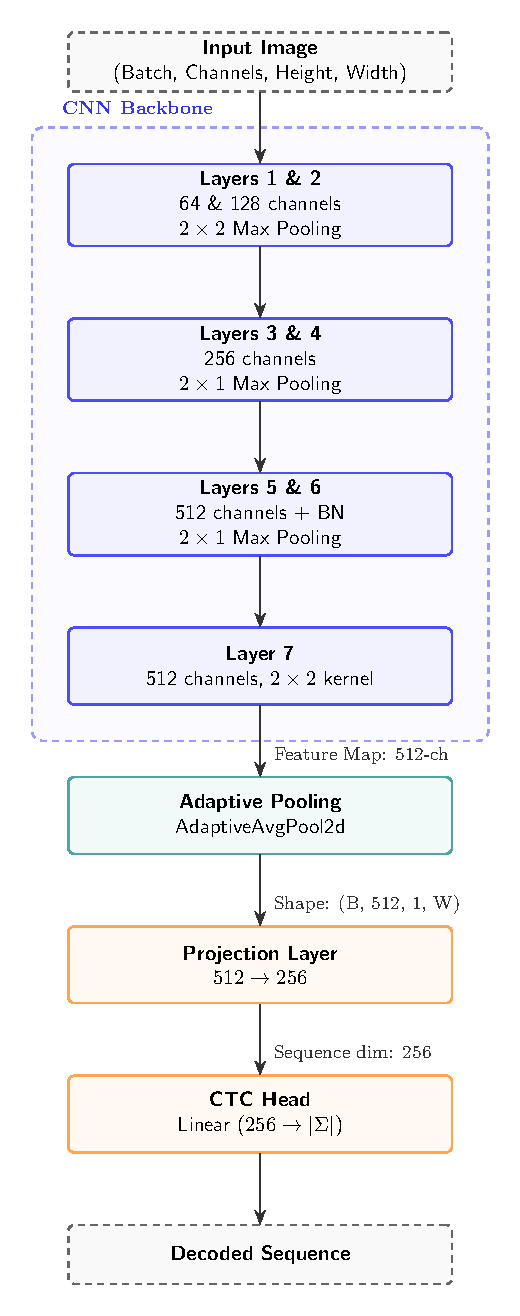
\includegraphics[width=0.85\linewidth]{figures/architecture_tikz.pdf}
\small CNN-CTC: 32$\times$800\,px input $\to$ CNN Backbone $\to$ Adaptive Pooling $\to$ Projection Layer $\to$ CTC head $\to$ Decoded Sequence.
}


% Methods / Methodology
% o Experimental setup
% o Workflow or algorithms
% o Diagrams and illustrations




% ------------------------------ COLUMN 2 ------------------------------
\column{0.34}



\block{2. Data, Methods \& Metrics}{
\textbf{Training} data was Spr\r{a}kbanken synthetic S\'{a}mi OCR dataset
(National Library of Norway), $\sim$307k line images (276k training + 31k hyperparameter tuning), 32$\times$800px. 


\vspace{8mm}
\textbf{Evaluation} data used \benchmarkSamples\ samples: \hfTestSamples\ in-domain synthetic lines (Spr\r{a}kbanken validation split) + \bookTestSamples\ parallel Northern S\'{a}mi--English sentences from Turi's 1910 "An Account of S\'{a}mi".

% \vspace{8mm}
% \begin{center}
%   
\includegraphics[width=0.95\linewidth]{figures/correct2.jpg}\\[2pt]
%   \footnotesize \textit{mij\'{a}v juohkkal\'{a}hk\'{a}j kreatijvvan.}
% \end{center}

% \begin{center}
%   
\includegraphics[width=0.95\linewidth]{figures/example1.jpg}\\[2pt]
%   \footnotesize \textit{sámi vuoigatvuođalaččaiguin, guoskevaš oasálaččaiguin}

%   \small Two Spr\r{a}kbanken synthetic samples shown as the model sees them.
% \end{center}
\vspace{8mm}
\textbf{Pipeline} - a lightweight, modular OCR$\rightarrow$MT:
\begin{enumerate}
  \item Image preprocessing (grayscale, 32$\times$800 px)
  \item 7-layer CNN backbone (64$\to$128$\to$256$^2$$\to$512$^3$ ch.)
  \item Adaptive pool + linear projection to 256 dimensions
  \item CTC decoder over a 395-symbol vocabulary
  \item Translation via TartuNLP API
\end{enumerate}
\vspace{8mm}
\textbf{Training.} AdamW (lr $10^{-4}$), batch 32, 100 epochs with early stopping, CTC loss, trained on a single NVIDIA V100. Inference benchmark on AMD Ryzen 5 PRO CPU.

\vspace{8mm}
\textbf{Negative result.} Pretrained VGG-16/19 and ResNet-50 backbones did not converge.

\vspace{8mm}
\textbf{Metrics Used.} \textbf{OCR:} Character Error Rate (CER), Word Error Rate (WER); Word Acc. $=100-$WER, Char Acc. measured directly ($\approx 100-$CER).

}


% Results and Findings
% o Graphs
% o Tables
% o Visual summaries

\block{3.1 Results: Benchmark}{

\textbf{Key result:} CNN-CTC achieves \ctcCacc\% accuracy (\ctcCER\% CER) with the fastest inference and smallest model.
\vspace{2mm}


% ---- Main benchmark table -------------------------------------------------
\begin{center}
\normalsize
\begin{tabular}{@{}lrrrr@{}}
\toprule
Model & \shortstack{Char.\\Acc.\ (\%)} & \shortstack{Word\\Acc.\ (\%)} & s/img & Size \\
\midrule
trocr\_smi\_synth$^\ast$         & \textbf{\trocrBestCacc} & \textbf{\trocrBestWordAcc} & \trocrBestTime  & \trocrSize \\
\textbf{ctc\_simple (ours)}      & \ctcCacc                 & \ctcWordAcc                 & \textbf{\ctcTime} & \textbf{\modelSize} \\
trocr\_smi\_pred\_synth$^\ast$   & \trocrPredSynthCharAcc   & \trocrPredSynthWordAcc      & \trocrPredSynthTime & \trocrSize \\
trocr\_smi                       & \trocrSmiCharAcc         & \trocrSmiWordAcc            & \trocrSmiTime    & \trocrSize \\
\bottomrule
\end{tabular}\\[1mm]
\footnotesize $^\ast$\texttt{smi}=S\'{a}mi data, \texttt{pred}=+auto-transcribed, \texttt{synth}=+synthetic pre-training.
\end{center}


% ---- Domain shift ---------------------------------------------------------
\vspace{20mm}
\begin{center}
\textbf{Generalization (in-domain vs. out-of-domain)}
\end{center}
\vspace{1mm}
\textbf{Key result:} TrOCR degrades by \trocrSynthDeltaCER\,pp, while CNN-CTC remains stable (\ctcCER\% $\rightarrow$ \ctcBookCER\%).

\begin{center}
\normalsize
\begin{tabular}{@{}lrrr@{}}
\toprule
Model & \shortstack{HF CER\\(\%)} & \shortstack{Book CER\\(\%)} & $\Delta$ (pp) \\
\midrule
trocr\_smi\_synth          & \textbf{\trocrSynthHFCER}  & \trocrSynthBookCER         & +\trocrSynthDeltaCER \\
\textbf{ctc\_simple (ours)}& \ctcCER                    & \ctcBookCER                & \textbf{-0.03} \\
trocr\_smi\_pred\_synth    & \trocrPredSynthHFCER       & \textbf{\trocrPredSynthBookCER} & -\trocrPredSynthDeltaCER \\
\bottomrule
\end{tabular}\\[1mm]
\footnotesize HF = in-domain, Book = historical out-of-domain.
\end{center}


% ---- Recognition example --------------------------------------------------


\vspace{20mm}
\begin{center}
\textbf{Example predictions (ground truth vs. prediction)}
\end{center}
\vspace{-10mm}
\begin{center}
\begin{tabular}{>{\centering\arraybackslash}p{\linewidth}}
\toprule
\textbf{Correct Recognition (CER = 0\%)} \\
\midrule
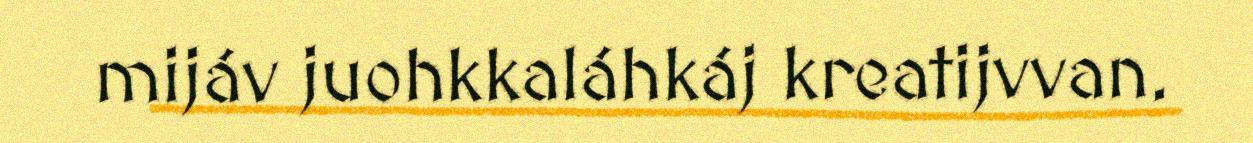
\includegraphics[width=0.92\linewidth]{./figures/ground_truth/correct2.jpg} \\
\small{\textbf{Ground Truth:}  \textit{mij\'{a}v juohkkal\'{a}hk\'{a}j kreatijvvan.}} \\
\small{
\textbf{Prediction:} \textit{mij\'{a}v juohkkal\'{a}hk\'{a}j kreatijvvan.}} \\[12mm]
\midrule
\textbf{Diacritical Errors (CER = 8.3\%)} \\
\midrule

\includegraphics[width=0.92\linewidth]{./figures/ground_truth/diacritical_errors_new.jpg} \\
\small{\textbf{Ground Truth:} \textit{ođđasis eal\'{a}skahttojuvvon) Suohkana h\'{a}lddahusla\v{s}}} \\ %\dj\dj 
\small{\textbf{Prediction:} \textit{oddasis eal\'{a}skahttojuvvon) Duohkama h\'{a}lddahusla\v{s}}} \\[12mm]
\midrule
\textbf{Uppercase Text Errors (CER = 29.6\%)} \\
\midrule

\includegraphics[width=0.92\linewidth]{./figures/ground_truth/uppercase_errors.jpg} \\
\small{
\textbf{Ground Truth:} \textit{FYLKKAGIELDDAIGUIN. FINNM\'{A}RKKU FYLKKAGIELDDAS LEA \'{A}IGUMU\v{S}\v{S}IEHTADUS S\'{A}MI}} \\
\small{
\textbf{Prediction:} \textit{FYLKKAGIELDDAIGUI0. F1O0m\'{A}RKKU FYLKKAGIELDDAs LEA \'{A}IGUmU\v{S}e}} \\
\bottomrule
\end{tabular}
\end{center}
}

% ------------------------------ COLUMN 3 ------------------------------
\column{0.33}


\block{3.2 Results: Other Findings}{
\vspace{-5mm}
\begin{center}
\textbf{Character accuracy vs.\ sentence length.}
\end{center}
The character accuracy drops for longer sentences due to the fixed
32$\times$800\,px input.\\



\centering
\vspace{-15mm}
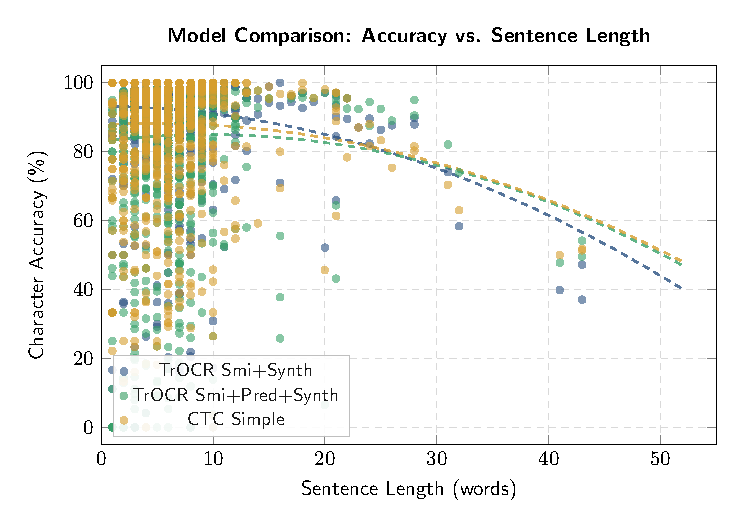
\includegraphics[width=0.85\linewidth]{figures/model_comparison_sentence_length.pdf}\\[2mm]
\vspace{-5mm}

% ---- Conjunction-splitting figure -----------------------------------------

\begin{center}
\textbf{Conjunction-based splitting on long sentences}
\end{center}

\flushleft
End-to-end OCR$\to$MT: On \bookTestSamples\ book sentences:
BLEU \bleuScore, chrF \chrfScore, TER \terScore.


\begin{center}
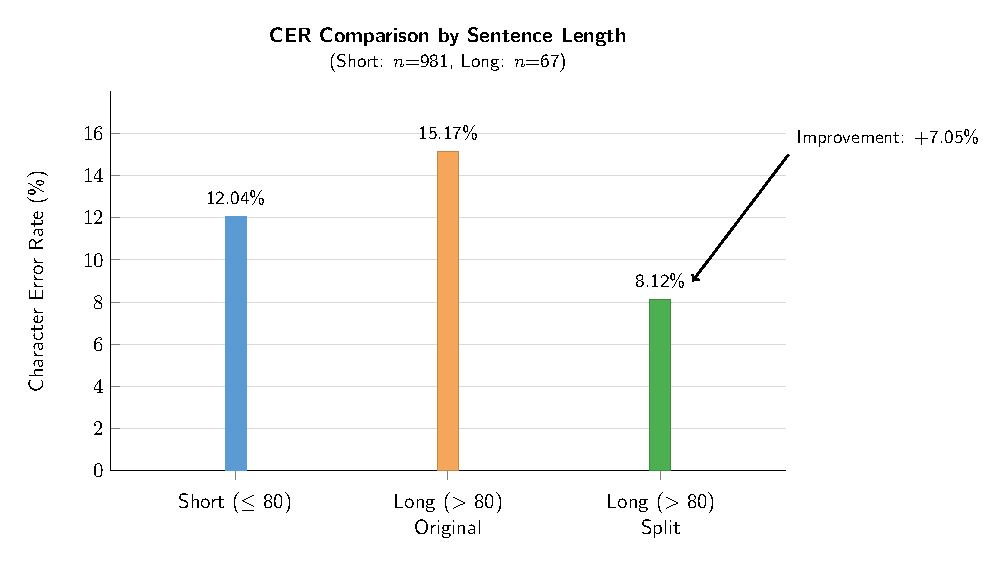
\includegraphics[width=0.9\linewidth]{figures/split_comparison.pdf}
\footnotesize{Linguistically motivated preprocessing splitting at S\'{a}mi conjunctions (\textit{ja}, \textit{muhto},
\textit{go}, \ldots) cuts long-sentence CER from \splitLongOriginalCER\%
to \splitLongSplitCER\%.}
\end{center}



}



% 5. Discussion / Conclusion
% o Key outcomes
% o Implications
% o Future work
\block{4.\ Conclusion \& Future Work}{


\textbf{Key Outcomes.} The CNN-CTC achieves \ctcCacc\% character accuracy. The evaluation accuracy barely moves between synthetic and historical book text (\ctcCER\% $\to$ \ctcBookCER\%). Yields an estimated throughput of $\sim$\throughputCtc\ img/h. The OCR$\to$MT pipeline achieves BLEU \bleuScore\ on the \bookTestSamples\ parallel sentences and conjunction-based splitting recovers $\sim$7\,pp CER on long sentences.

\textbf{Implications.} The CNN-CTC model trails the best TrOCR by only \cerAccGap\,pp
character accuracy while being roughly \sizeRatio$\times$ smaller and \speedupFactor$\times$ faster, making it worthwhile for resource-constrained deployment. The in and out of domain accuracy stability lacks sufficient statistical power for concrete conclusions but it might suggest better lightweight generalisation. The MT quality indicates the need for improved English translation models for S\'{a}mi. Conjunction-based splitting proved to be a valid preprocessing proof-of-concept.

\textbf{Future Work:} Use real scanned documents, layout analysis for full-page processing, morphological post-correction, mobile / edge deployment for field digitization

\centering
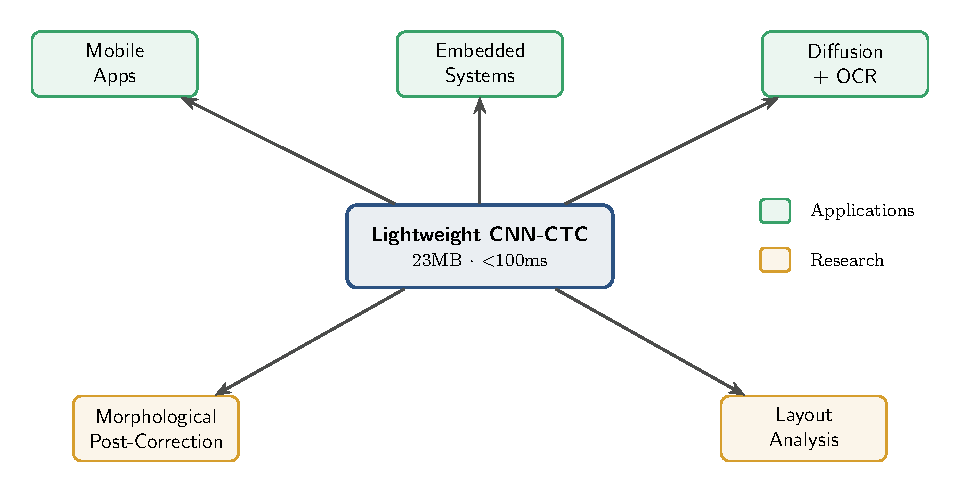
\includegraphics[width=0.95\linewidth]{figures/future_work.pdf}
\footnotesize Future work: real scans, layout analysis, morphological post-correction, mobile deployment.
}

\block{References \& Acknowledgments}{
\footnotesize
\textbf{Key references.}
[1] Enstad et al.\ \emph{Comparative analysis of OCR for S\'{a}mi}, NoDaLiDa 2025. 
[2] Li et al.\ \emph{TrOCR}, AAAI 2023.

[3] Shi et al.\ \emph{CRNN}, IEEE TPAMI 2017.

[4] Corallo \& Varde, \emph{OCR for Amazigh}, AAAI Workshops 2023.

[5] Turi, \emph{Muitalus s\'{a}miid birra}, 1910.

[6] TartuNLP MT API, 2025.\\[3mm]

\textbf{Acknowledgments.} A.\ Varde acknowledges grant NNF25OC0110035 (Denmark).\\[2mm]
% \url{https://github.com/magwrap/north-sami-ocr}
% \begin{minipage}[c]{0.48\linewidth}\centering
\begin{center}
  \textbf{Code:} \url{https://github.com/magwrap/north-sami-ocr} \\
  
\includegraphics[width=0.15\linewidth]{figures/github-qr-code.png}
\end{center}
% \end{minipage}
}

\end{columns}

\end{document}